
\section{Introdução}


\begin{frame}

\begin{center}
{\huge Capítulo 1 -- Introdução}\\
(Contexto e Motivação aos SMAS)
\end{center}

\end{frame}

\begin{frame}

  \frametitle{Rápido Histórico da IA $\Rightarrow$  IAD $\Rightarrow$ SMA}
    
\begin{itemize}
  \item IA cresceu muito nos anos $70 \rightarrow 80 ...$
   modelando a inteligência individual.
  \item  Advento das redes de computadores modificou as necessidades!
  \item  Inteligência como a integração dos processos de \textit{raciocinar},    \textit{decidir}, \textit{aprender} e  \textit{planejar}.
  \item  O \textit{Modelo de Agente} aparece então como catalisador...
\end{itemize}


\end{frame}

%-----------------------------------------------------------------------
\begin{frame} %[allowframebreaks=0.9]

 \frametitle{Em verdade:}

\begin{itemize}
  \item Mundo onde informações e conhecimentos crescem (e mudam) rápido demais!
    \item O crescimento da Internet trás desafios constantes que incluem:
    \begin{itemize}
  \item Acesso a informações relevantes
  \item Identificação de oportunidades
    \item Ação no momento preciso
  \item Manipulação de grandes volumes de informação
\end{itemize}
 \item Ubiqüidade, Gerenciamento e Inteligência
\end{itemize}

\end{frame}
%-----------------------------------------------------------------------


%-----------------------------------------------------------------------
\begin{frame} %[allowframebreaks=0.9]

 \frametitle{Encaminhando aos SMAs}
\begin{itemize}
  \item  Vários problemas não podem mais serem tratados 
  de modo \textcolor{red}{\textbf{centralizado}}, por exemplo:
  \begin{itemize}
    \item Controle de linha de trens (Brasil) metrô (hum SP talvez)
    \item Monitoramento de Redes de Computador
    \item Diagnóstico Médico
    \item Compra e Venda

  \end{itemize}

\pause  
\item Como Resolvê-los?\\
\pause
\underline{Inteligência Coletiva} $ \Rightarrow $ \underline{IA Distribuída}  $ \Rightarrow $

\begin{itemize}
  \item Resolução Distribuída de Problemas (RDP)
  \item Sistemas Multiagentes (SMA) $\Leftarrow $ \textcolor{red}{foco deste curso}
\end{itemize}
\end{itemize}

\end{frame}
%-----------------------------------------------------------------------

\begin{frame}

  \frametitle{Motivando aos SMAs}
    
    
\begin{figure}[!ht]
\centering
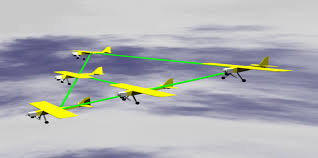
\includegraphics[height =.6\textheight,width=.7\textwidth]{figuras/agentes_vizinhos01.jpeg}
\caption{Observe o sentido das flechas --  e  o foco da missão}
%\label{ag_01}
\end{figure}
    
    
\end{frame}

%-----------------------------------------------------------------------

\begin{frame}
\frametitle{Motivando aos SMAs}

\begin{figure}[!ht]
\centering
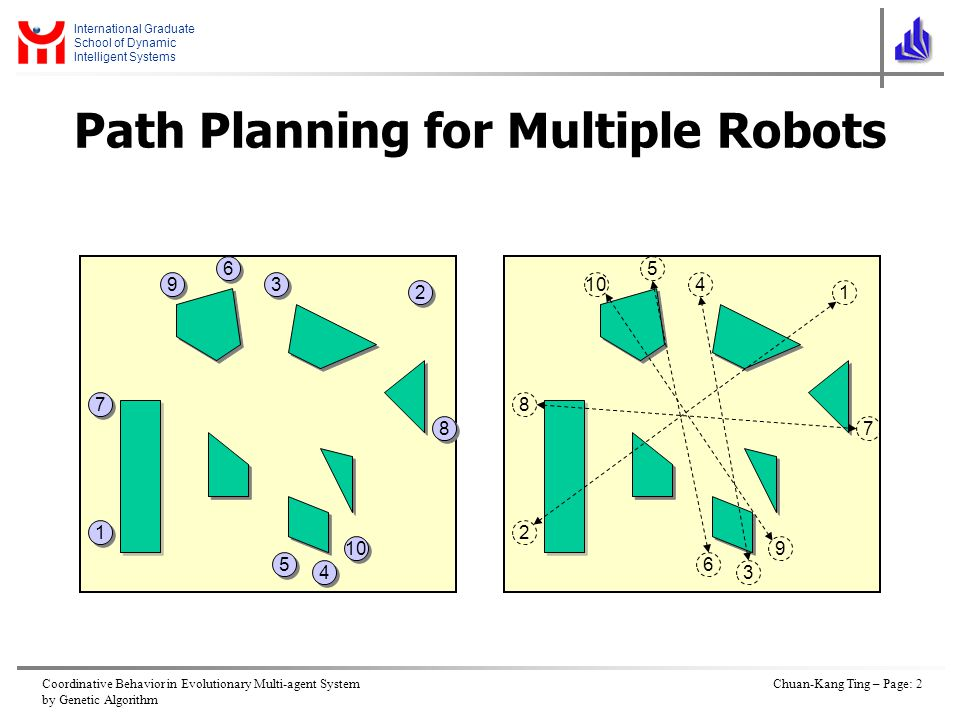
\includegraphics[height =.6\textheight,width=.7\textwidth]{figuras/agentes_vizinhos02.jpeg}
%\caption{Arquitetura clássica}
%\label{ag_01}
\end{figure}
\end{frame}

%-----------------------------------------------------------------------

\begin{frame}

  \frametitle{Motivando aos SMAs}

\begin{figure}[!ht]
\centering
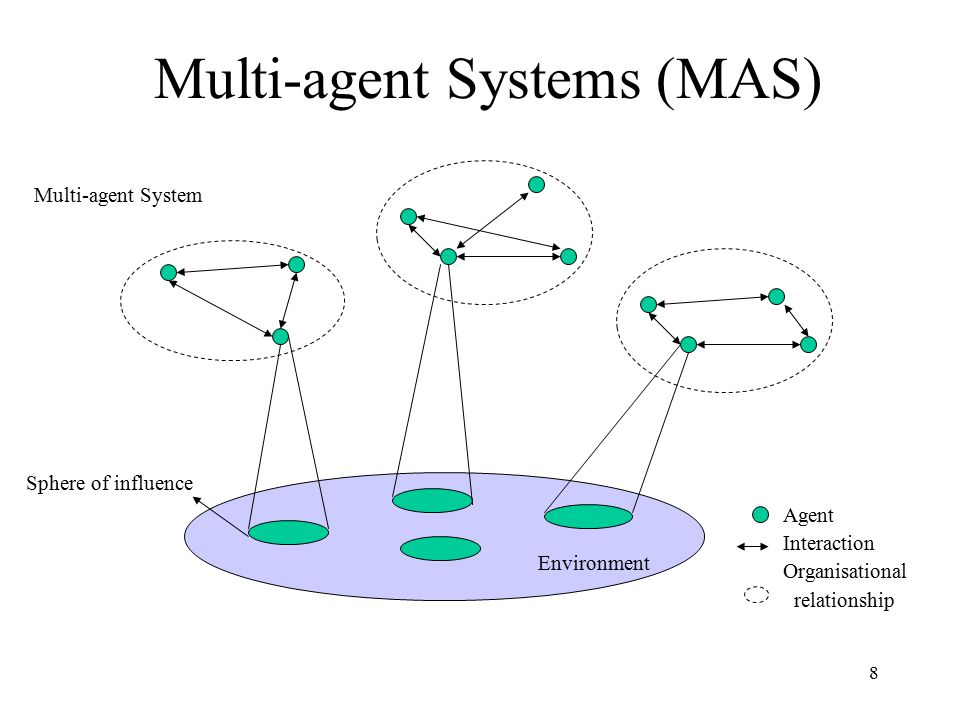
\includegraphics[height =.7\textheight,width=.8\textwidth]{figuras/agentes_vizinhos03.jpeg}
\caption{Visão clássica de SMAs -- comunidade de agentes $\equiv $ SMA}
%\label{ag_01}
\end{figure}
 
\end{frame}
%%%%%%%%%%%%%%%%%%%%%%%%%%%%%%%%%%%%%%%%%%%%%%%%%%%%%%%%%%%%%%%%%


\subsection{Motivação aos SMAs}
\begin{frame} %%%[allowframebreaks=0.9]

\frametitle{Motivação I}
    Projetar e construir sistemas multiagentes é uma tarefa difícil, pois:
 \begin{itemize}
   \pause
   \item Apresenta todos os problemas já conhecidos 
dos sistemas distribuídos e concorrentes.
   \pause
   \item Dificuldades adicionais surgem da flexibilidade 
e complexidade das interações
    \end{itemize}
\end{frame}


%--------------------------------------

\begin{frame}
\frametitle{Problemas de tabuleiro são simples?}
  
  \begin{figure}[!ht]
  \centering
  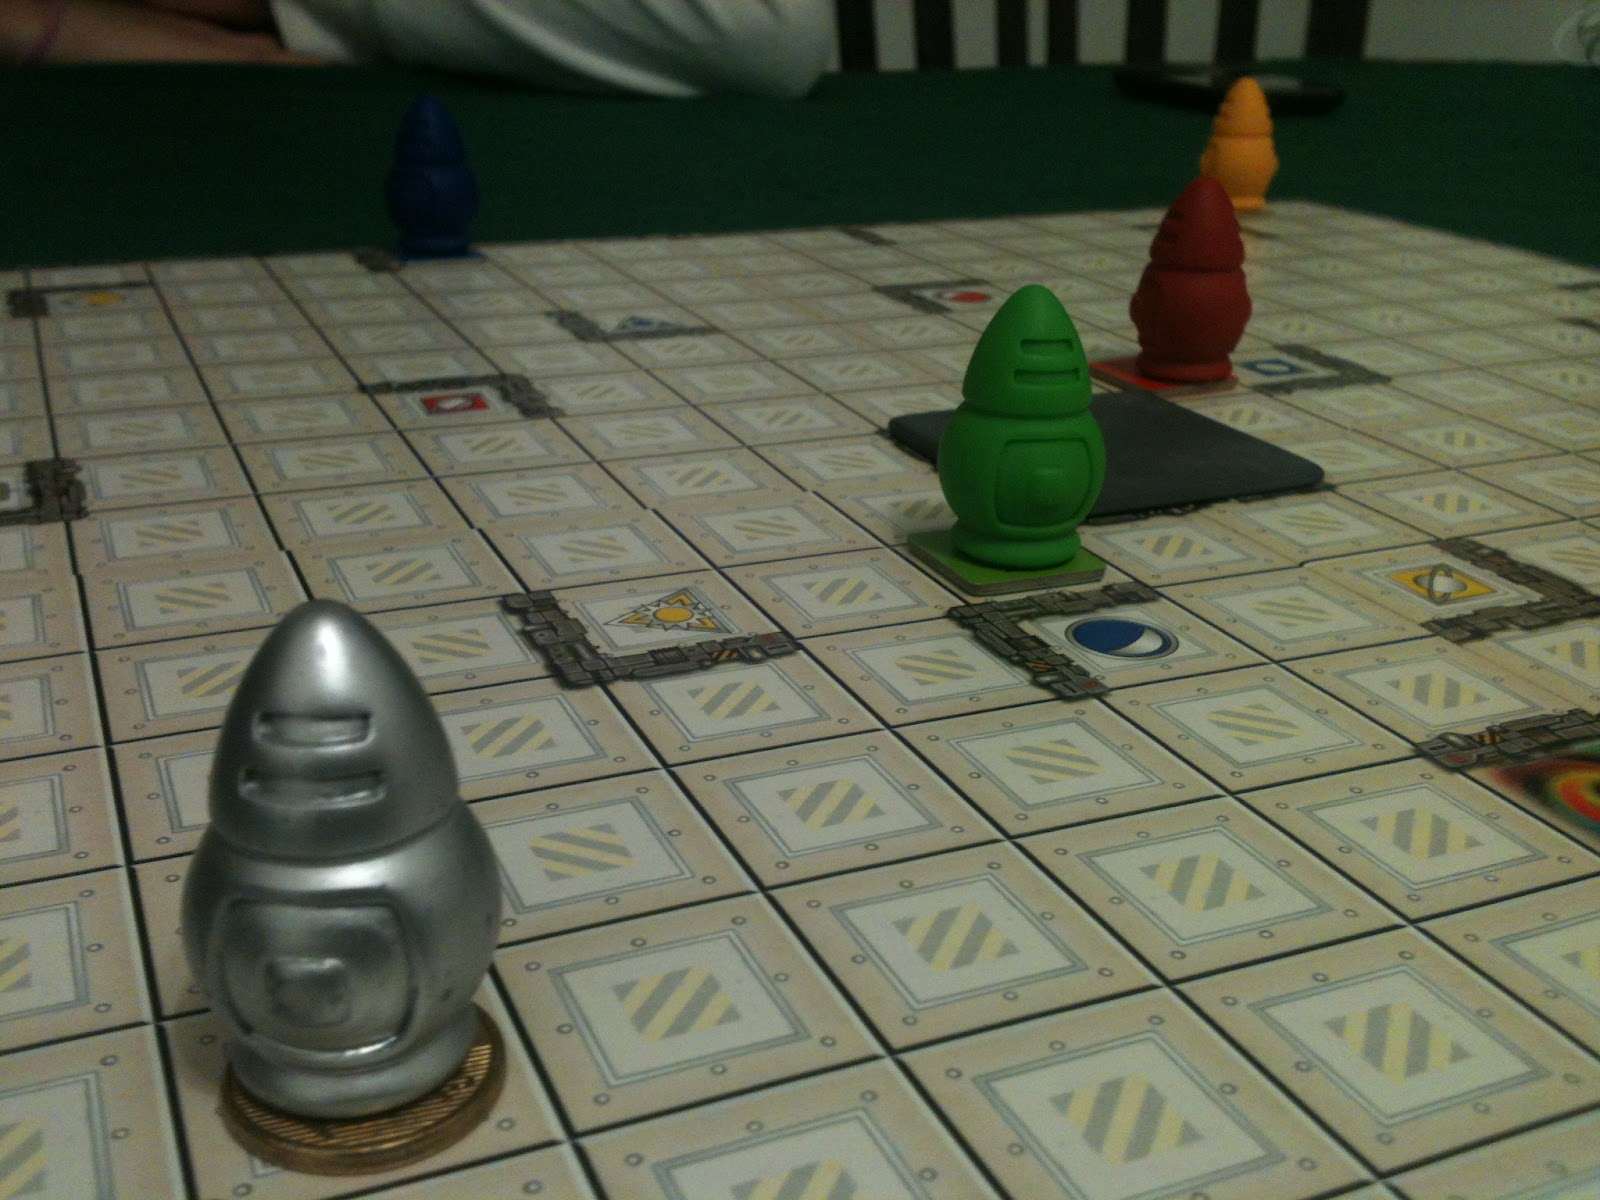
\includegraphics[height =.6\textheight,width=.7\textwidth]{figuras/robos_tabuleiro.jpg}
  \caption{Admita um robo indo de uma posição inicial ($S_0$) há uma final 
  ($S_m$)}
%\label{ag_01}
\end{figure}
   
\end{frame}

%----------------------------------------------------------

\begin{frame}
\frametitle{Exemplificando a complexidade por um DFD com  \textbf{um agente} 
$\times$ \textbf{n-ações}:}
  
  \begin{figure}[!ht]
  \centering
  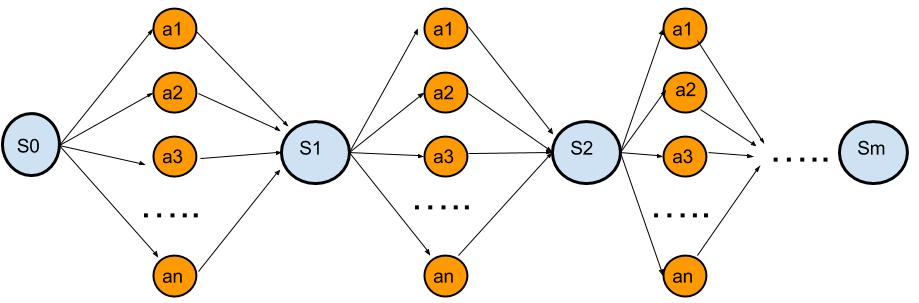
\includegraphics[height =.6\textheight,width=.9\textwidth]{figuras/dfd_simples_acoes.jpg}
  \caption{Complexidade via DFD de um agente $\times $ ações $\equiv $ um estado  inicial ($S_0$) há um estado final ($S_m$)}
%\label{ag_01}
\end{figure}
   
\end{frame}

%----------------------------------------------------------

\begin{frame}
\frametitle{Exemplificando a complexidade por um DFD por \textbf{agentes} $\times$ \textbf{ações}:}
  
  \begin{figure}[!ht]
  \centering
  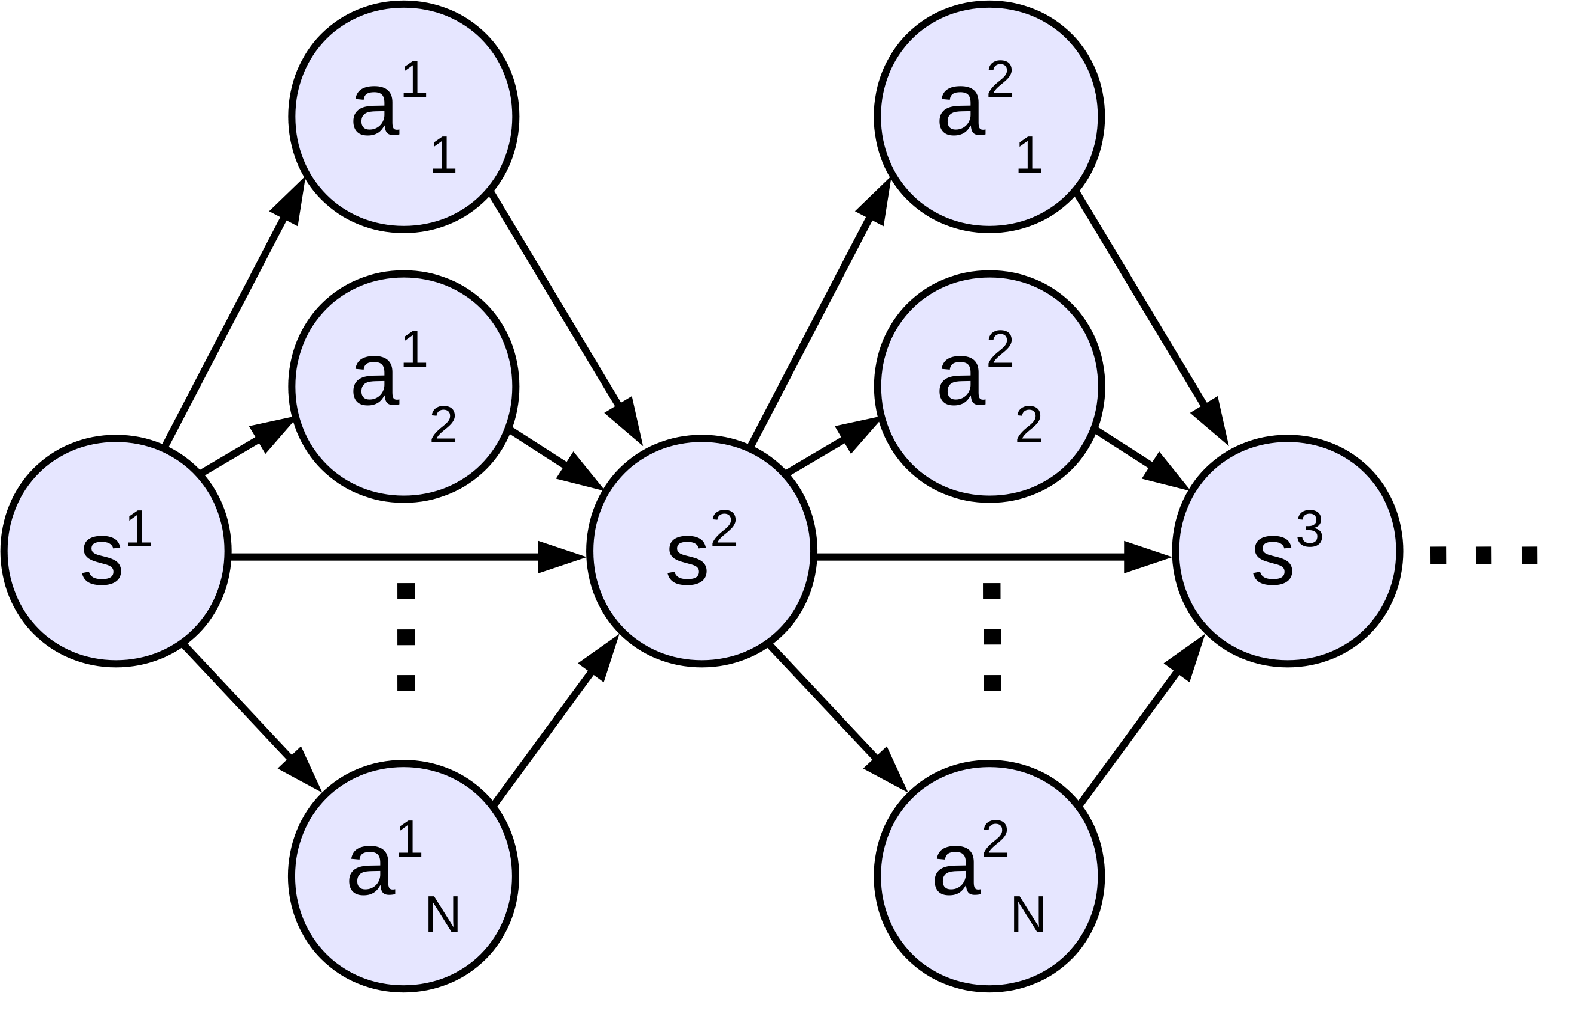
\includegraphics[height =.6\textheight,width=.8\textwidth]{figuras/mudando_estados01.png}
  \caption{Complexidade via DFD de um SMA (agentes) $\times $ ações $\equiv $ um único estado}
%\label{ag_01}
\end{figure}
   
\end{frame}

%----------------------------------------------------------

\begin{frame}

\frametitle{Exercício -- papel e caneta mesmo}
   
\begin{block}{}

  \begin{itemize}
  \item Considere que as ações sejam do tipo um deslocamento de uma célula. 8 direções ou 4?
  \pause
  \item Considere que o robô não vai ficar em ciclos -- passar em estados que já passou -- fácil isto? Como resolver?
  \pause
  
  \item   Para as duas versões acima estime a complexidade dos mesmos em número
  de combinações possíveis de um $S_0$ há um $S_m$.
  \pause
  
   \item Introduza as dimensões do tabuleiro em seus cálculos e refaça-os
  \end{itemize}  
  
\end{block}
   
\end{frame}



%----------------------------------------------------------
\begin{frame}

    \frametitle{Motivação II -- retomando ...}
   Dois principais impedimentos técnicos, pois:
  \begin{itemize}
  \pause
  \item Inexistência de uma metodologia sistemática para 
      claramente especificar e estruturar aplicações SMA.
  \pause
  \item Inexistência de ferramentas e ambientes de 
desenvolvimento de SMA com qualidade industrial.
    
  \end{itemize}

\end{frame}

%----------------------------------------------------------
%%%%%%%%%%%%%%%%%%%%%%%%%%%%%%%%%%%%%%%%%%%%%%%%%%%%%%%%%%%%%%%%%%%%%%%%

\subsection{Os Elementos de SMAs}

\begin{frame}%%%[allowframebreaks=0.9]

 \frametitle{Os Elementos de SMAs}
  
  \begin{block}{O que abordaremos neste curso:}
  
   \begin{description}
  
     \item[Projeto de Agente:] \textbf{\textcolor{red}{... ao longo do curso}}
     
    \item[Ambiente:] \textbf{\textcolor{red}{... ao longo do curso}}
          
   \item[Percepção:] \textbf{\textcolor{red}{... ao longo do curso}}
               
 \item[Controle:] \textbf{\textcolor{red}{... ao longo do curso}}
                    
  \item[Conhecimento:] \textbf{\textcolor{red}{... ao longo do curso}}
                          
  \item[Comunicação:] \textbf{\textcolor{red}{... ao longo do curso}}
          
   \end{description}
  \end{block}    
   
\end{frame}
%-------------------------------------------------



\begin{frame}

\frametitle{Exercício}
   
\begin{figure}[!ht]
\centering
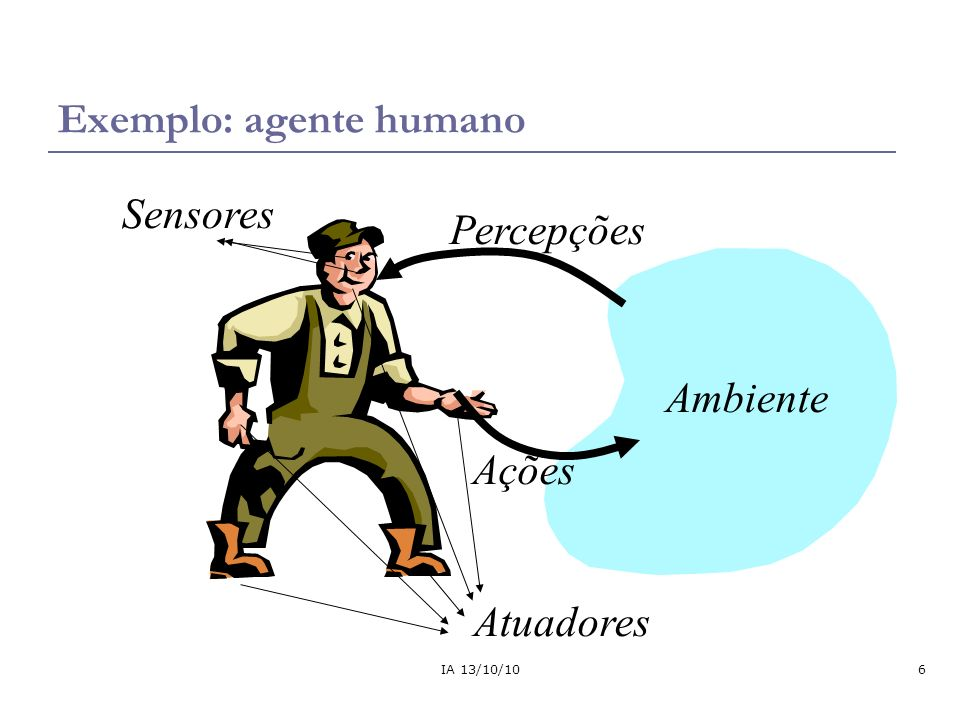
\includegraphics[height =.6\textheight,width=.7\textwidth]{figuras/agente_humano.jpg}
\caption{Exercício: enumere domínios para este agente identificando os itens de SMAs}
%\label{ag_01}
\end{figure}

   
\end{frame}



%%%%%%%%%%%%%%%%%%%%%%%%%%%%
